\section{fork-2.c}

	Muestre la pantalla de ejecucución del programa:

	\begin{center}
		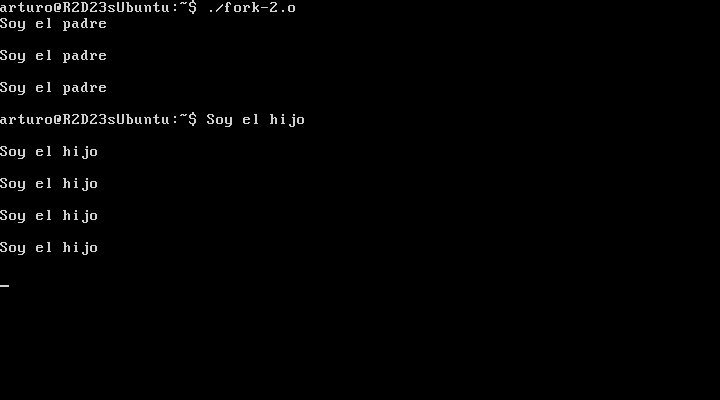
\includegraphics[width=\linewidth]{imagenes/fork-2.png}
	\end{center}

	Responda lo siguiente:

	\begin{itemize}

		\item ¿La variable n toma dos valores diferentes, dependiendo del proceso que se ejecute, o se tiene una variable n para cada proceso (padre e hijo)?\\
		Se tiene una variable para cada proceso.
		\item Explique el por qué de su respuesta a la pregunta anterior.\\
		El programa imprime un número diferente de mensajes dependiendo si el proceso que lo corre es el padre o el hijo. Esto implica que dicha variable ostenta valores diferentes.

	\end{itemize}
